\documentclass[../main.tex]{subfiles}

\begin{document}

\section{Sharing the Filesystem}
\label{section:lauxus:sharing}

% WHY = need root key for accessing the FS. currently root key is sealed on the owner computer. With property of sealing we are stuck. Need an out of band channel to transmit an encrypted version of the root key as depicted in figure ...
\par Now that we have seen how LAUXUS works on a local computer, we can dig on the sharing capabilities. As we have seen, the root key is the key material for accessing the Filesystem. Currently, we know that it is sealed on the owner computer. This allows to bind the root key to his computer. Indeed, once a material is sealed with SGX, the only party that can unseal it is the SGX instance that sealed it in the first place. This means that we can't just share the sealed version of the root key to other users. As we depicted in the Figure \ref{figure:lauxus:approach}, we need an out of band channel for transmitting the encrypted version of the root key. This is what we will cover in this Section.

% before going further, lets recall the every users owns a public / private asymmetric key pair -> allows other to verify that a message a truly been sent by a specific user. this will be proven helpful in our case
\par Before going further, lets remember that currently every user owns an asymmetric ECC key pair allowing other users to authenticates a message sent by another users (we consider that all the public keys are securely accessible for all the users). This functionality will become handy in our protocol.

% protocol will be based on ECDH enabling ... For this we will use ephemeral ECDH key pairs enabling the following equation (when we know the pk of the destination user)
% In a nutshell protocol will be splitted in 4 phases:
%   BY SENDER AND RECEIVER: creating a message attestating that we are using a correct SGX. Plus we will create a new key binding the user to the machine (user key and enclave key specific to this computer and only known to itself)
%   BY SENDER: testify RECEIVER OK and extract his public enclave key
%   BY SENDER: derive a shared secret between the ephemeral key and the pk enclave
%   BY RECEIVER: same as step 2 but reverse
%   BY RECEIVER: can derive the same shared secret and decrypt the RK before sealing (binding it to the machine)
\medbreak
\par The sharing protocol is based on the ECDH (Elliptic Curve Diffie-Hellman) particularity. ECDH enables to compute a secret from two key-pairs. Mathematically, if we have two key-pairs: $(pk_1, sk_1)$ and $(pk_2, sk_2)$, a shared secret K can be computed in the following way:
\begin{equation}
    \label{equation:lauxus:ecdh_secret}
    K = ECDH\_SECRET(pk_1, sk_2) = ECDH\_SECRET(pk_2, sk_1)
\end{equation}
With \textit{ECDH\_SECRET} being a know algorithm in the Elliptic Curve domain.
\par In practice, this means that: two users can securely compute the same secret just by knowing the public key of the other user.


\medbreak
\par As terminology, we will use the same user as in the Figure \ref{figure:lauxus:approach}. This means that Alice will share the root key with Carl. In a nutshell, the protocol will be splitted in 4 phases:
\begin{enumerate}
    \item Alice and Carl will create a message attesting that they are using a valid SGX Enclave. This message will also binds the user to its machine. This message will be called: the \textit{authenticity message}.
    \item Alice will checks the authenticity and the validity of the \textit{authenticity message} created by Carl.
    \item Alice will derive a shared secret (this secret is bind to this root key transaction) using the Equation \ref{equation:lauxus:ecdh_secret}. She will then encrypt the root key with this secret and share the result with Carl.
    \item Carl will checks the authenticity and the validity of the \textit{authenticity message} created by Alice.
    \item Carl will derive the same shared secret as Alice and will then be able to decrypt the root key before sealing it on his computer.
\end{enumerate}
\par What this all means is that: Alice will encrypt the root key that only Carl can decrypt. This encryption key is unique and bind to both users and both users computer. This means that every time Carl is using a different computer, the protocol must be re-run.


\subsubsection{Phase 1 - Creating the \textit{authenticity message}}
\begin{figure}[h]
    \centering
    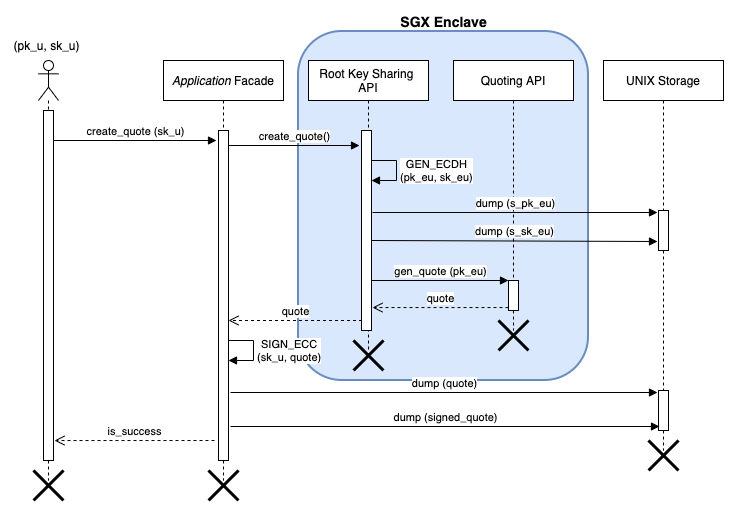
\includegraphics[width=\textwidth]{../../images/lauxus/create_quote}
    
    \caption{Phase 1 Sequence Diagram}
    \label{figure:lauxus:create_quote}
\end{figure}
\par The Figure \ref{figure:lauxus:create_quote} explains the first Phase and is based on the Quoting capability of SGX Enclaves (cfr. Chapter \ref{chapter:theoric}). In order to bind the user to his computer, we create another key-pair\footnote{pk\_eu stands for the public key of the user U's Enclave - similar notation with the secret key} inside the Enclave and seal them. The quote bears the Enclave public key and the quote is signed using the user private key for authentication.

\subsubsection{Phase 2 - Verifying the \textit{authenticity message}}
\begin{figure}[ht]
    \centering
    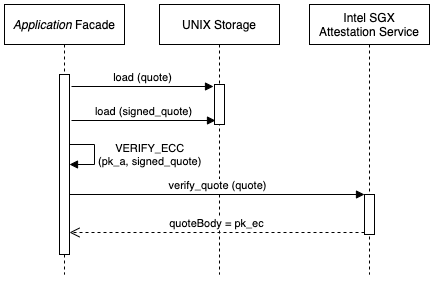
\includegraphics[width=.75\textwidth]{../../images/lauxus/verify_quote}
    
    \caption{Phase 2 Sequence Diagram}
    \label{figure:lauxus:verify_quote}
\end{figure}
\par The Figure \ref{figure:lauxus:verify_quote} explains the second Phase and is based on the remote Intel Attestation Service furnished by Intel (cfr. Chapter \ref{chapter:theoric}). Upon success, the initiator will be sure that this specific user is using a valid SGX Enclave.

\subsubsection{Phase 3 - Encrypting the root key for sharing}
\begin{figure}[ht]
    \centering
    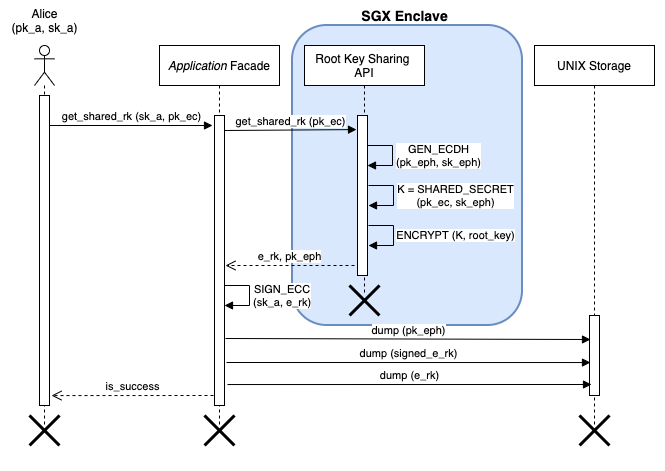
\includegraphics[width=\textwidth]{../../images/lauxus/upload_rk}
    
    \caption{Phase 3 Sequence Diagram}
    \label{figure:lauxus:upload_rk}
\end{figure}
\par The Figure \ref{figure:lauxus:upload_rk} explains the third Phase which is made by the administrator one time for each other user (if the other user never changes his computer). As explained in the Sequence Diagram, Alice creates an ephemeral key-pair\footnote{pk\_eph stands for ephemeral key-pair - similar notation with the secret key}. The encrypted root key is signed with Alice private key in order to testify authenticity.

\subsubsection{Phase 4 - Decrypting the shared root key}
\begin{figure}[ht]
    \centering
    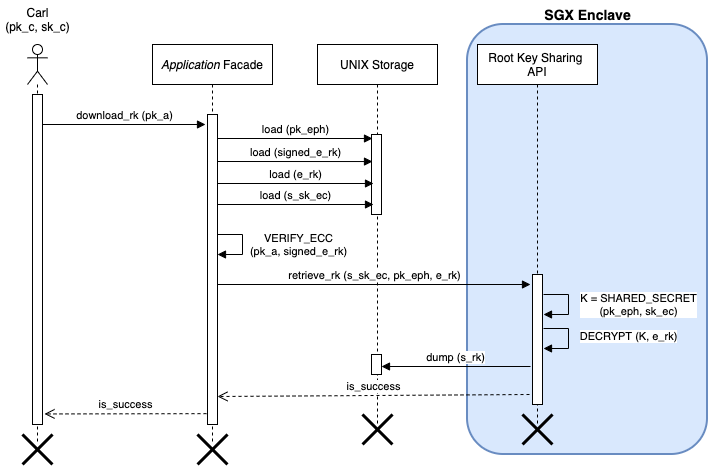
\includegraphics[width=\textwidth]{../../images/lauxus/download_rk}
    
    \caption{Phase 4 Sequence Diagram}
    \label{figure:lauxus:download_rk}
\end{figure}
\par The Figure \ref{figure:lauxus:download_rk} explains the fourth and final Phase which is straightforward knowing the third Phase. We just need to do the opposite operation. The shared secret reconstructed thanks to the ephemeral public key.



% BIG SYNTHESIS

\end{document}